% 2008 年北京卷理科第 8 题：正方体 ABCD-A1B1C1D1，P 在体对角线 BD1 上，
%   过 P 作垂直于平面 BB1D1D 的直线，与正方体表面交于 M、N。
% 来源 PDF：gaokaomath-src/普通高考/2008/2008北京理.pdf
% SHA-256：1ba43840bfc822e6bcd4a1c04e69becd857890f1abf3da09910b4f26ae25c9a8
% 原页：2008北京理.pdf 第 1 页（A3 三栏）第 1 栏，书页码 425。
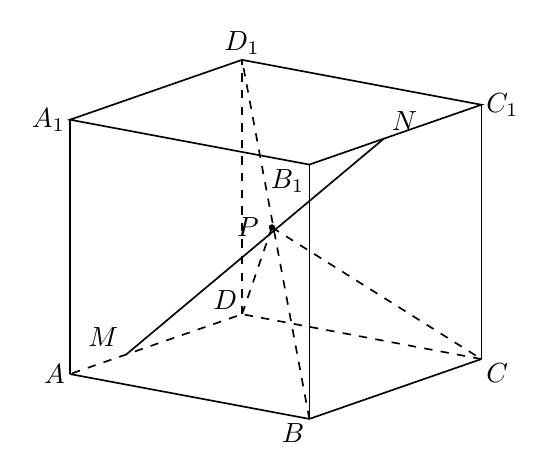
\begin{tikzpicture}[scale=0.95, semithick,
  every node/.style={inner sep=1.5pt}]
  \coordinate (A) at (0.0,0.9);
  \coordinate (B) at (3.2,0.3);
  \coordinate (C) at (5.5,1.1);
  \coordinate (D) at (2.3,1.7);
  \coordinate (A1) at (0.0,4.3);
  \coordinate (B1) at (3.2,3.7);
  \coordinate (C1) at (5.5,4.5);
  \coordinate (D1) at (2.3,5.1);

  \draw (A) -- (B) -- (C);
  \draw[dashed] (C) -- (D) -- (A);
  \draw (A) -- (A1);
  \draw (B) -- (B1);
  \draw (C) -- (C1);
  \draw (A1) -- (B1) -- (C1) -- (D1) -- cycle;
  \draw[dashed] (D) -- (D1);
  \draw[dashed] (B) -- (D1);

  % P 与过 P 的 MN（平行 AC）
  \coordinate (P) at (2.7,2.86);
  \coordinate (M) at (0.75,1.16);
  \coordinate (N) at (4.2,4.05);
  \draw (M) -- (N);
  \fill (P) circle (1.2pt);
  \draw[dashed] (P) -- (D);
  \draw[dashed] (P) -- (C);

  \node[left] at (A) {$A$};
  \node[below left] at (B) {$B$};
  \node[below right] at (C) {$C$};
  \node[above left] at (D) {$D$};
  \node[left] at (A1) {$A_1$};
  \node[below left] at (B1) {$B_1$};
  \node[right] at (C1) {$C_1$};
  \node[above] at (D1) {$D_1$};
  \node[left=3pt] at (P) {$P$};
  \node[above left=1pt] at (M) {$M$};
  \node[above right=1pt] at (N) {$N$};
\end{tikzpicture}
